\clearpage

\subsection{Edytor zapytań SQL wykonywanych natychmiast}

Edytor zapytań SQL wykonywanych natychmiast to jeden z najważniejszych elementów
programu. Pozwala administratorowi na wygodne edytowanie, testowanie i
wykonywanie natywnych zapytań SQL. 

Interfejs komponentu składa się z edytora zapytań, edytora zapytania testowego i
przycisków służących do wykonywania lub testowania zapytań.

Wybranie opcji ``Commit'' powoduje wykonanie zapytania w transakcji, która
zostanie zatwierdzona, gdy wszystkie zapytania zostaną wykonane bez błędów.
Wybranie opcji commit nie pokaże administratorowi informacji zwrotnych poza
informacją, czy wykonanie zapytań przebiegło pomyślnie.

Wybranie opcji ``Test'' spowoduje wykonanie transakcji, która zostanie wycofana
przed zwróceniem danych wynikających z zapytań SQL. Dane wynikające z zapytań z
listy zapytań zostaną wyświetlone pod odpowiednim zapytaniem.

Jeśli administrator zaznaczył opcję ``Diff test query'', dane wynikające z
zapytania testowego zostaną wyświetlone w specjalnym oknie pod tekstem zapytania
testowego z możliwością przełączania pomiędzy wynikiem zapytania przed
wykonaniem listy zapytań i po wykonaniu listy zapytań. Interfejs widać na
rysunku \ref{testQueryBeforeAfterFigure}.

Jeśli administrator zaznaczył opcję ``Diff mermaid.js ER diagram'', program
wygeneruje diagram ER tabel w bazie danych przed wykonaniem listy zapytań i po
wykonaniu listy zapytań. Diagramy zostaną pokazane w specjalnym oknie z
możliwością przełączania pomiędzy diagramem przed wykonaniem listy zapytań i po
wykonaniu listy zapytań oraz z możliwością pokazania diagramu w trybie
pełnoekranowym. Porównanie widać na rysunku \ref{diagramBeforeAfterFigure}, a
widok pełnoekranowy widać na rysunku \ref{diagramFullscreenFigure}.

Edytor składa się z listy pól tekstowych, gdzie administrator może wpisywać
pojedyncze zapytania SQL. Administrator może dodawać nowe pola tekstowe,
zmieniać kolejność pól, kasować pola i wyłączać pola. Pola wyłączone nie będą
wykonywane. Jest to przydatne do testowania wpływu wykonania zapytania na wynik
kolejnych zapytań.

\begin{figure}[h]
    \centering
    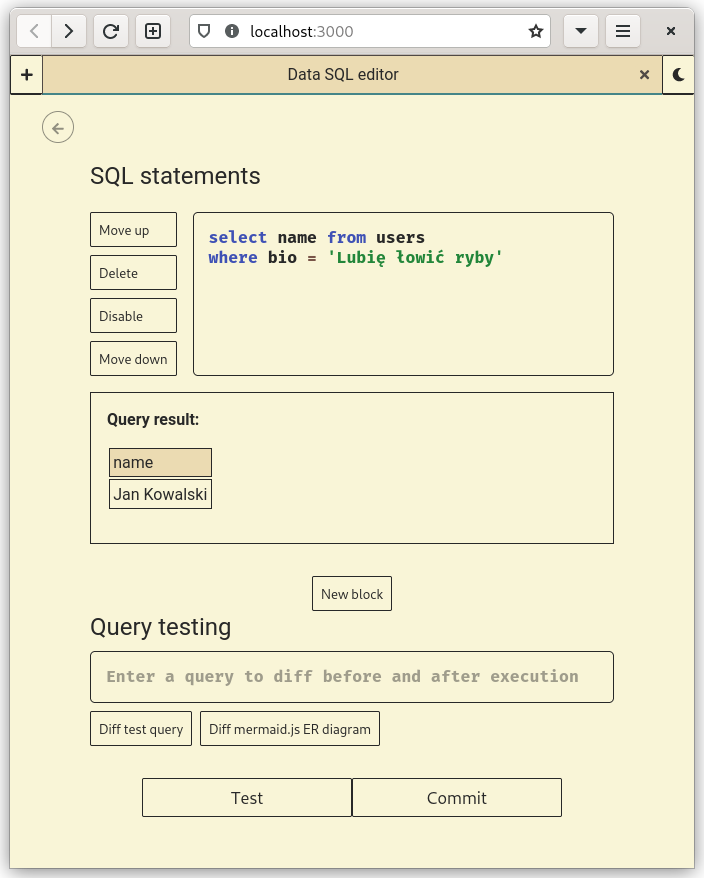
\includegraphics[width=0.6\textwidth]{./img/sql_editor.png}
    \caption{Edytor SQL wykonywanego natychmiast}
    \label{immediateSqlEditorFigure}
\end{figure}

\begin{figure}
    \centering
    \subfloat[\centering Przed wykonaniem]
        {{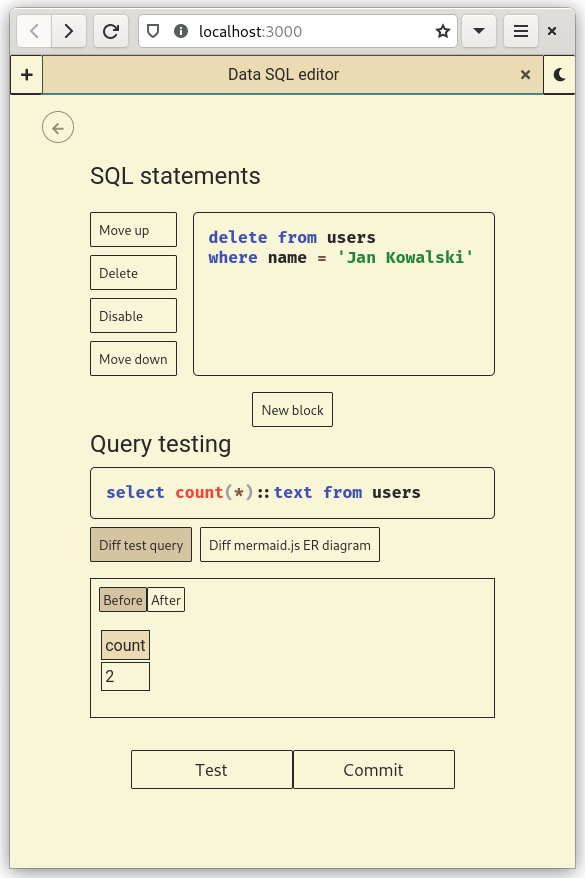
\includegraphics[width=6cm]{./img/test_query_before.png} }}
    \qquad
    \subfloat[\centering Po wykonaniu]
        {{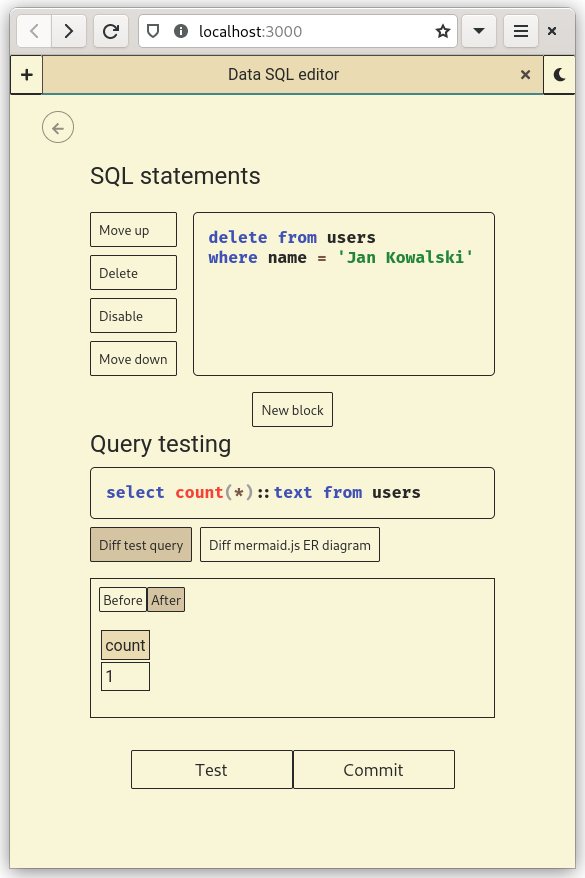
\includegraphics[width=6cm]{./img/test_query_after.png} }}

    \caption{Porównanie zapytania testowego}
    \label{testQueryBeforeAfterFigure}
\end{figure}

\begin{figure}
    \centering
    \subfloat[\centering Przed wykonaniem]
        {{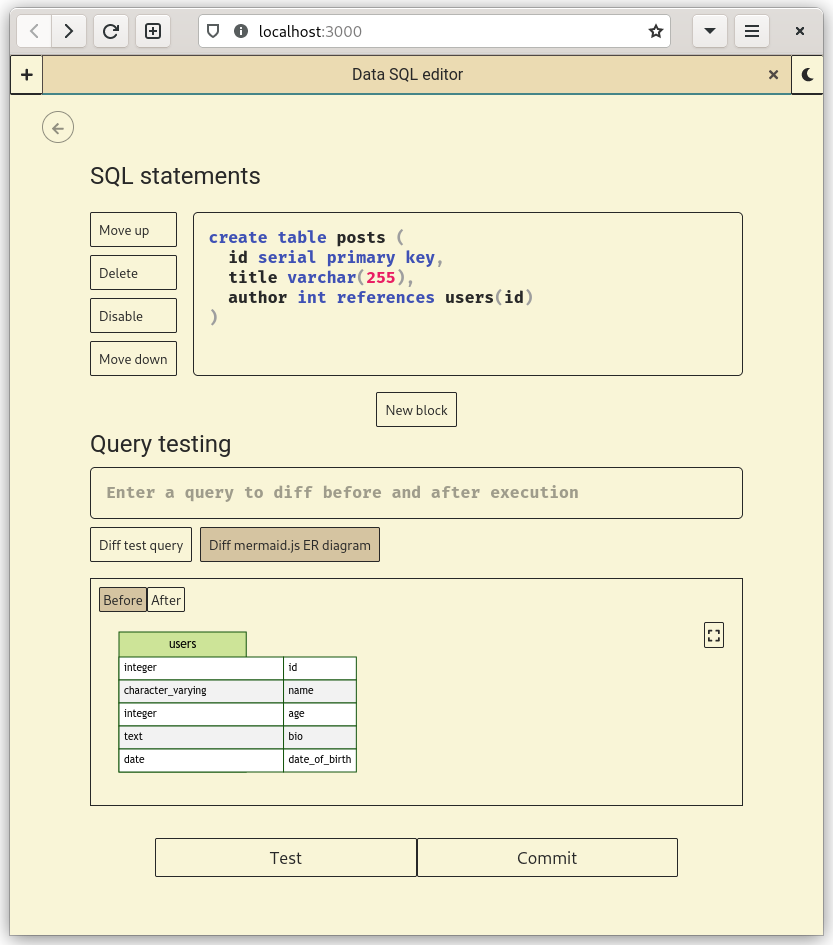
\includegraphics[width=.47\textwidth]{./img/diagram_diff_before.png} }}
    \qquad
    \subfloat[\centering Po wykonaniu]
        {{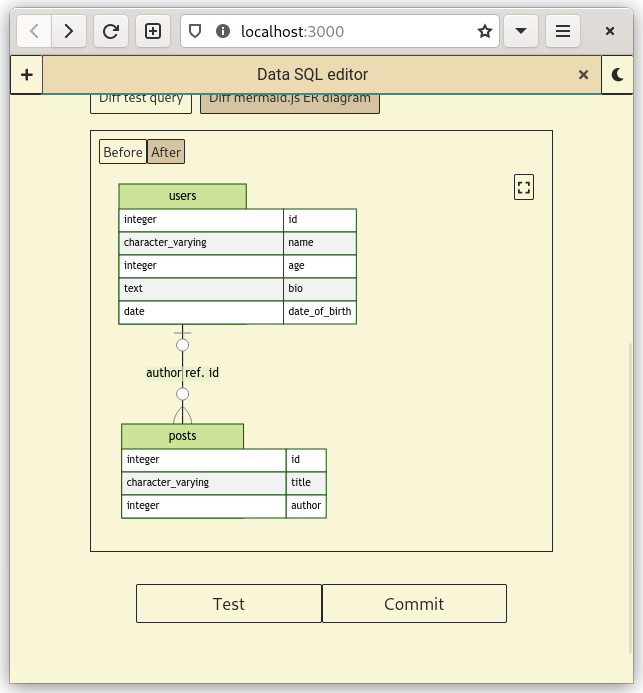
\includegraphics[width=.47\textwidth]{./img/diagram_diff_after.png} }}

    \caption{Porównanie diagramu ER}
    \label{diagramBeforeAfterFigure}
\end{figure}

\begin{figure}[h]
    \centering
    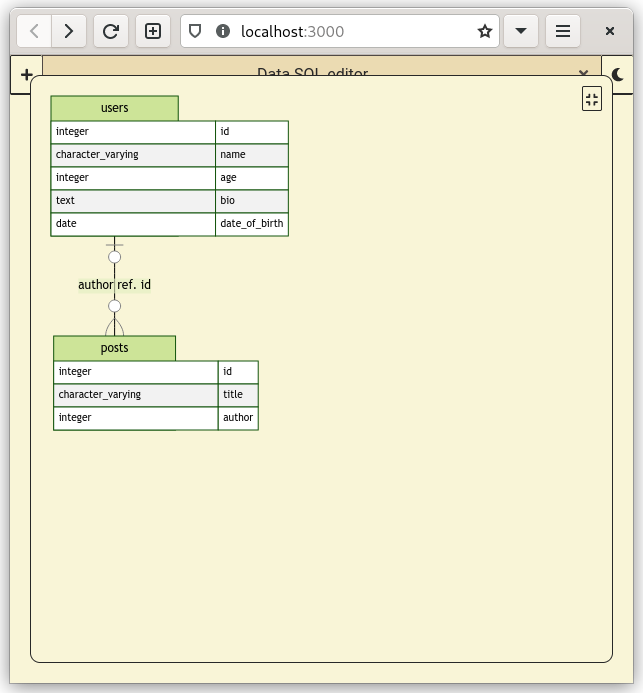
\includegraphics[width=0.6\textwidth]{./img/diagram_diff_after_fullscreen.png}
    \caption{Widok pełnoekranowy diagramu}
    \label{diagramFullscreenFigure}
\end{figure}
